\documentclass[aps,prb,twocolumn,superscriptaddress,floatfix,longbibliography]{revtex4-2}

\usepackage[utf8]{inputenc}
\usepackage[spanish]{babel}
\usepackage{graphicx}
\usepackage{amsmath}
\usepackage{subcaption}
\usepackage{wrapfig} 
\usepackage[export]{adjustbox}

\usepackage{amsmath,amssymb} % math symbols
\usepackage{bm} % bold math font
\usepackage{graphicx} % for figures
\usepackage{comment} % allows block comments
\usepackage{textcomp} % This package is just to give the text quote '
%\usepackage{ulem} % allows strikeout text, e.g. \sout{text}

\usepackage[spanish]{babel}

\usepackage{enumitem}
\setlist{noitemsep,leftmargin=*,topsep=0pt,parsep=0pt}

\usepackage{xcolor} % \textcolor{red}{text} will be red for notes
\definecolor{lightgray}{gray}{0.6}
\definecolor{medgray}{gray}{0.4}

\usepackage{hyperref}
\hypersetup{
colorlinks=true,
urlcolor= blue,
citecolor=blue,
linkcolor= blue,
bookmarks=true,
bookmarksopen=false,
}

% Code to add paragraph numbers and titles
\newif\ifptitle
\newif\ifpnumber
\newcounter{para}
\newcommand\ptitle[1]{\par\refstepcounter{para}
{\ifpnumber{\noindent\textcolor{lightgray}{\textbf{\thepara}}\indent}\fi}
{\ifptitle{\textbf{[{#1}]}}\fi}}
\ptitletrue  % comment this line to hide paragraph titles
\pnumbertrue  % comment this line to hide paragraph numbers

% minimum font size for figures
\newcommand{\minfont}{6}

% Uncomment this line if you prefer your vectors to appear as bold letters.
% By default they will appear with arrows over them.
% \renewcommand{\vec}[1]{\bm{#1}}

%Cambiar Cuadros por Tablas y lista de...
%\renewcommand{\listtablename}{Índice de tablas}
\renewcommand{\tablename}{Tabla}
\renewcommand{\date}{Fecha}

\usepackage[bottom]{footmisc} %para que las notas al pie aparezcan en la misma página



\begin{comment}

%Comandos de interés:

* Para ordenar el documento:
\section{Introducción}
\section{\label{sec:Formatting}Formatting} %label para luego hacer referencia a esa sección

\ptitle{Start writing while you experiment} %pone nombre y título al documento dependiendo de si en el header están los comandos \ptitletrue y \pnumbertrue

* Ecuaciones:
\begin{equation}
a^2+b^2=c^2 \,.
\label{eqn:Pythagoras}
\end{equation}

* Conjunto de ecuaciones:
\begin{eqnarray}
\label{eqn:diagonal}
\nonumber d & = & \sqrt{a^2 + b^2 + c^2} \\
& = & \sqrt{3^2+4^2+12^2} = 13
\end{eqnarray}

* Para hacer items / enumerar:
\begin{enumerate}
  \item
\end{enumerate}

\begin{itemize}
  \item
\end{itemize}

* Figuras:
\begin{figure}[h]
    \includegraphics[clip=true,width=\columnwidth]{pixel-compare}
    \caption{}
     \label{fig:pixels}
\end{figure}

* Conjunto de figuras:
(no recuerdo)


* Para hacer referencias a fórmulas, tablas, secciones, ... dentro del documento:
\ref{tab:spacing}

* Para citar
Elementos de .bib
\cite{WhitesidesAdvMat2004}
url
\url{http://www.mendeley.com/}\\

* Agradecimientos:
\begin{acknowledgments}
We acknowledge advice from Jessie Zhang and Harry Pirie to produce Fig.\ \ref{fig:pixels}.
\end{acknowledgments}

* Apéndice:
\appendix
\section{\label{app:Mendeley}Mendeley}

* Bibliografía:
\bibliography{Hoffman-example-paper}

\end{comment}

\begin{comment}

Plots y tablas en orden:

* Figura de los cilindros con los PT100, la resistencia de referencia, la fuente, el multímetro y la computadora simbolizando el software de adquisisción de datos.
* Figura de los cilindros con la lampartira, la fuente que le da tensión y el multímetro para medir esa tensión

* Tabla de dimensiones de los cilindros
(la copio de prácticos anteriores)

* Figura del equipo de algto vacío (bomba mecánica, difusora, tubos, bridas, cámara, 3 cilindros...)
* Figura sobre cómo determinar epsilon (pirómetro, termocupla apoyados sobre cilindro exterior sin vacío)

PLOT PPAL:
* T vs t mostrando un gráfico lindo donde se vea bien el transitorio y el estacionario

SUBPLOTS:
* T vs t mostrando qué pasa si hay un cortocircuito interno que hace que la lámpara no prenda (se ven T bajas)
* T vs t mostrando qué pasa si no ponemos el telgopor
* T vs t mostrando qué pasa si falla el vacío
* T vs t mostrando qué pasa en el cilindro externo cuando agregamos N2
* T vs t mostrando qué pasa cuando cambiamos la potencia de la lamparita sobre la marcha



Determinación del producto de ctes
* T vs P recta para calcular la pendiente relacionada con el producto de constantes

Determinación de epsilon
* Gráfico Epsilon vs P

Bibliografía:
* Agregar referencia a la tabla de calibración R vs T
* Agregar referencia a que sacamos los datos de las áreas de un práctico de años anteriores

\end{comment}



\begin{document}

% Allows to rewrite the same title in the supplement
\newcommand{\mytitle}{Análisis computacional del modelo Issing en 2 dimensiones}

\title{\mytitle}

\author{Pablo Chehade \\
    \small \textit{pablo.chehade@ib.edu.ar} \\
    \small \textit{Física computacional, Instituto Balseiro, CNEA-UNCuyo, Bariloche, Argentina} \\}



\begin{abstract}
Se analizó computacionalmente el modelo Issing en dos dimensiones en un sistema finito con condiciones de contorno periódicas. Se emplearon condiciones inciales aleatorias y la evolución del sistema quedó determinada por el algoritmo de Metrópolis. En primer lugar, se analizó la evolución de la energía por espín y la magnetización por espín para temperaturas menor, mayor y cercana a la temperatura de Curie, definida como aquella en la que ocurre la transición ferromagnética. En segundo lugar, se analizó el estado transitorio para un ensamble de sistemas a distintas temperaturas. Esto permitió caracterizar el cambio de fases ferromagnético a través de un diagrama de fases. Por último, bajo las mismas condiciones se calculó la capacidad calorífica a partir de la variación de energía en el estado estacionario. Analizando el diagrama de fases y la capacidad calorífica, se determinó experimentalmente la temperatura de Curie y se comparó con el valor analítico $T_c^{teo} = 2.269185$ en unidades de $1/k$, $k$ constante de Bolzmann. A partir del diagrama de fases se obtuvo $T_c^1 = 1.9$ con una discrepancia del $ 16 \%$. Mientras que a partir de la capacidad calorífica se obtuvo $T_c^2 = 2.22$ con una discrepancia del $ 2\%$.


\end{abstract}

\maketitle

\section{Motivación}

El modelo Ising es un modelo físico que busca explicar el ferromagnetismo. Es ampliamente estudiado en la Mecánica Estadística y si bien fue concebido inicialmente para estudiar el magnetismo, actualmente es de utilidad en varios campos de la física. Por ejemplo, se lo ha utilizado para estudiar el movimiento de los átomos (Lattice gas) y el comportamiento de una red neuronal (Hopfield), entre muchas otras aplicaciones.

\section{Introducción}

El modelo Ising en dos dimensiones consta de un sistema de espines ${s_i}$ que a efectos prácticos se considera un ensamble canónico. Dichos espines se encuentran arreglados en los nodos de una red bidimensional de tamaño $N \times N$ y pueden tomar dos valores posibles: $s_i = +1$ o $-1$, correspondientes a $\uparrow$ o $\downarrow$. La evolución del sistema está dada por varios factores. En primer lugar, la condición inicial. En segundo lugar, una interacción de corto alcance entre cada espín y sus vecinos, lo cual determina la energía magnética total del sistema a través de la expresión $E = - J \sum_{{i j \in <nn>}} s_i s_j$, con $J>0$. En tercer lugar, las fluctuaciones de energía dadas por el intercambio con el medio.

La evolución del sistema está caracterizada por variaciones considerables de la energía durante las primeras iteraciones en un proceso denominado termalización. Luego de cierto tiempo $t_{max}$ se alcanza el estado estacionario caracterizado por pequeñas fluctuaciones de energía. El valor de la magnetización $M$ en el estado estacionario es el que determina las propiedades magnéticas del sistema: si todos los espines se encuentran en el mismo estado, el sistema se encuentra en la fase ferromagnética. La magnetización se define a partir de la expresión $M = \mu \sum_{i_1}^{N^2} s_i$ y la magnetización por esín, $m = M/{N^2}$. Experimentalmente se obtiene que la fase ferromagnética se da a temperaturas bajas. Al aumentar la temperatura ocurre una transición de fase hacia un estado caracterizado por espines en estados aleatorios con magnetización total nula. Esta transición ocurre a una temperatura determinada denominada temperatura de Curie ($T_c$) y corresponde al máximo de la derivada de $d|m|/dT$.


Además, desde el punto de vista termodinámico, dicha transición está caracterizada por la divergencia de la capacidad calorífica, definida como
\begin{equation}
c(m, H) = \left( \frac{\partial E}{\partial T}  \right)_H = \frac{\sigma_E^2}{k T^2},
\label{eq:capacidad_calorifica}
\end{equation}
donde $H$ es el campo aplicado, $\sigma_E$ las fluctuaciones de energía en el estado estacionario y $k$ la constante de Boltzmann. Es importante aclarar que esta cantidad diverge a $T = T_c$ sólo en un sistema bidimensional infinito. Para sistemas finitos se esperaría a dicha temperatura un máximo creciente con $N$.

En el presente trabajo se simuló computacionalmente el modelo Ising sin campo externo en un sistema bidimensional finito. Se estudió la evolución de la energía por espín y la magnetización por espín, además de la transición ferromegnética por medio de un diagrama de fases y de la divergencia de la capacidad calorífica. Se consideró $J = 1$, $k = 1$ y $\mu = 1$, de modo que $T$ se expresa en unidades de $1/k$.

\section{Método experimental}

\begin{figure}[h]
    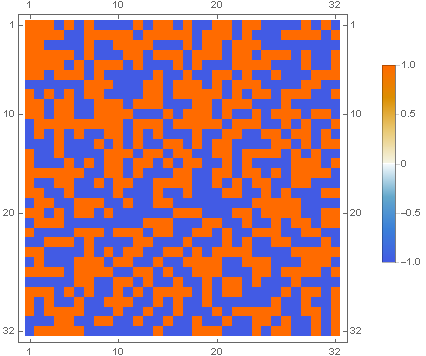
\includegraphics[clip=true,width=\columnwidth]{condicion_inicial.png}
    \caption{Condición inicial aleatoria para red de tamaño $N = 32$.}
     \label{fig:condicion_inicial}
\end{figure}

Se empleó una red bidimensional periódica de tamaño $N \times N$ con condición inicial aleatoria, como la retratada en la figura \ref{fig:condicion_inicial}. La evolución temporal fue simulada mediante el algoritmo de Metrópolis. Este algoritmo da una regla de evolución probabilística en la que la probabilidad $p$ de que un espín cambie de estado es
\[p = min(1,e^{-\Delta E / k T})\]
donde $\Delta E$ es la variación de energía correspondiente al cambio de estado. En la implementación del algoritmo se empleó el paso de Monte Carlo, aplicando aleatoriamente la regla de evolución a $N^2$ espines para cada paso de tiempo.

En base a lo anterior, se estudió la evolución del sistema, focalizándose en el análisis de la transición de fase. En primer lugar, se analizó la evolución temporal de la energía por espín y la magnetización por espín para tres temperaturas: $T = 1.5$, $1.85$ y $5$ en un sistema de tamaño $N = 32$. En segundo lugar, se construyó el diagrama de fases. Para esto se simuló a distintas temperaturas un ensamble de $M = 30$ sistemas con tamaño de red $N = 8$ y se midió en cada uno de ellos $|m|$ y $\sigma_{|m|}$ en el estado estacionario, considerando que el proceso de termalización finaliza en $t_{max} = 10 N$. Se empleó una red de tamaño menor de modo que el programa se ejecute en un tiempo razonable. Realizando el promedio de ensambles, el valor medio del módulo de la magnetización ( $\langle |m| \rangle$ ) y la desviación estándar correspondiente ( $\sigma_{\langle |m| \rangle}$ ) quedan determinadas por las expresiones

\begin{equation}
\langle |m| \rangle = \frac{1}{M} \sum_{k = 1}^{M} |m_k|
\label{eq:ensamble_m}
\end{equation}

\begin{equation}
\begin{split}
\sigma^2_{\langle |m| \rangle} & = \sigma_{dispersion}^2 + \sigma_{desviacion}^2 \\
& = \frac{1}{M} \sum_{k=1}^M (|m_k| - \langle |m| \rangle)^2 + \frac{1}{M} \sum_{k=1}^M \sigma_{|m_k|}^2,
\end{split}
\label{eq:ensamble_sigma_m}
\end{equation}

donde $\sigma_{dispersion}$ da cuenta de la dispersión de los valores $|m_{k}|$ obtenidos, y $\sigma_{desviacion}$, del error en la determinación de cada $|m_{k}|$.

En tercer lugar, para un ensamble de $M = 40$ sistemas de tamaño $N = 5$ se midió la desviación estándar de la energía por espín $\sigma_E$, de modo de determinar la capacidad calorífica mediante la expresión \ref{eq:capacidad_calorifica}.


\section{Resultados y discusión}

\subsection{Evolución temporal}

En primer lugar, para las temperaturas $T = 1.5$, $1.85$ y $5$ se obtuvo la dependencia de la energía por espín y la magnetización por espín graficadas en las figuras \ref{fig:energia_vs_t.png} y \ref{fig:mag_vs_t.png}, respectivamente. Se observa a simple vista que el sistema logra termalizar a $t = t_{max}$. Para $T=1.5$ se observa que el sistema alcanza rápidamente el estado estacionario caracterizado por $m$ cercana a 1. Esto se observa claramente en el estado final del sistema graficado en la figura \ref{fig:final_T_1.5}, donde gran parte de los espines se encuentran en el mismo estado. Por simetría, $m$ no tiene preferencia por el estado $+1$ o $-1$, de modo que la elección de un estado u otro es aleatoria. En base a lo anterior, lo correcto es estudiar el módulo $|m|$.

\begin{figure}[h]
    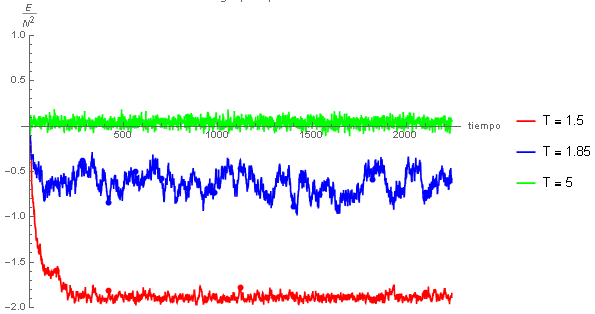
\includegraphics[clip=true,width=\columnwidth]{energia_vs_t.png}
    \caption{Evolución temporal de la energía por espín para distintas temperaturas.}
     \label{fig:energia_vs_t.png}
\end{figure}

\begin{figure}[h]
    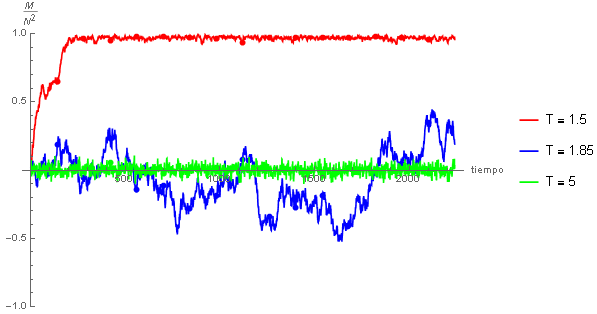
\includegraphics[clip=true,width=\columnwidth]{mag_vs_t.png}
    \caption{Evolución temporal de la magnetización por espín para distintas temperaturas.}
     \label{fig:mag_vs_t.png}
\end{figure}

\begin{figure}[h]
    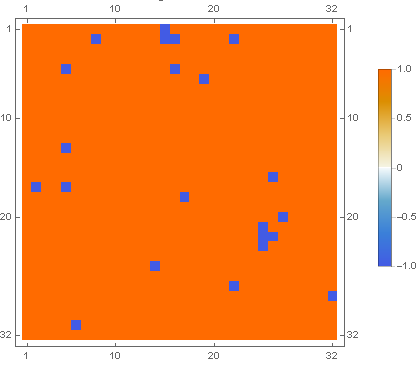
\includegraphics[clip=true,width=\columnwidth]{final_T_1.5.png}
    \caption{Sistema a temperatura $T = 1.5$ a $t = 2240$ pasos.}
     \label{fig:final_T_1.5}
\end{figure}


Aumentando la temperatura a $T= 1.85$ se observa que el sistema alcanza un estado estacionario caracterizado por grandes variaciones de la energía respecto al caso anterior y una magnetización no definida. Esto último en el sentido de que a pesar de que se llega al estado estacionario, $m$ continúa variando en el tiempo, oscilando alrededor del valor nulo. Esto se observa también en el estado final graficado en la figura \ref{fig:final_T_1.85}, donde los espines están distribuídos en ambos estados, con mayor cantidad en el estado 1 correspondiente a $m>1$. Nótese que en este caso se forman cúmulos de espines con un mismo estado.

\begin{figure}[h]
    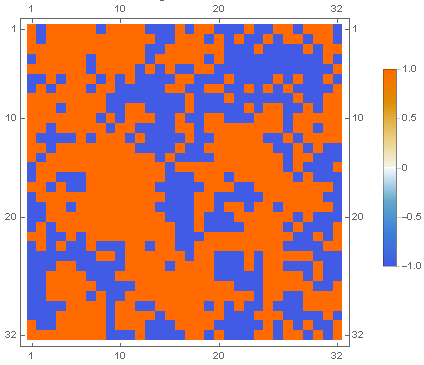
\includegraphics[clip=true,width=\columnwidth]{final_T_1.85.png}
    \caption{Sistema a temperatura $T = 1.85$ a $t = 2240$ pasos.}
     \label{fig:final_T_1.85}
\end{figure}

Aumentando nuevamente la temperatura a $T = 5$ se obtiene un sistema con energía cercana a cero en el estado estacionario y magnetización nula. Esto se refleja en espines distribuídos aleatoriamente en los posibles estados, como se verifica en la figura \ref{fig:final_T_5}.

\begin{figure}[h]
    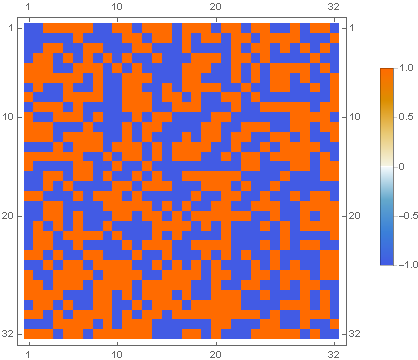
\includegraphics[clip=true,width=\columnwidth]{final_T_5.png}
    \caption{Sistema a temperatura $T = 5$ a $t = 2240$ pasos.}
     \label{fig:final_T_5}
\end{figure}

Claramente se está en presencia de un fenómeno crítico: a determinada $T$ el sistema en el estado estacionario cambia su comportamiento. Comienza con $|m| = 1$ para temperaturas bajas y alzanza $|m| = 0$ para temperaturas altas.

\subsection{Diagrama de fases}
Para caracterizar el fenómeno crítico se analizó $|m|$ en el estado estacionario para un rango de temperaturas, considerando no un único sistema sino un conjunto de ellos denominado ensamble. Se obtuvieron los resultados graficados en la figura \ref{fig:diagrama_de_fases}. En primer instancia, se observa el mismo comportamiento descripto anteriormente. En segunda instancia, se obtiene que la dispersión aumenta progresivamente hasta ser máxima en la región central y disminuir progresivamente para temperaturas mayores. Como vimos anteriormente, la dispersión en la región central es consecuencia de que $m$ no estabiliza en el estado estacionario.

Realizando un promedio de los valores obtenidos para cada $T$ mediante la ecuación \ref{eq:ensamble_m} y calculando los errores correspondientes a través de la expresión \ref{eq:ensamble_sigma_m}, se obtiene el diagrama de fases de la figura \ref{fig:diagrama_de_fases_pro}. En este se logra caracterizar tanto la variabilidad de $|m|$ en el estado estacionario para cada sistema, como la dispersión de la misma variable entre los sistemas de un ensamble. Como se mencionó anteriormente, la transición ocurre a la temperatura de Curie, la cual corresponde al máximo de la derivada de $ d|m|/dT$. En función de esto, se obtiene $T_c^1 = 1.9$. La discrepancia con el valor analítico $T_c^{teo} = 2.269185$ es del $ 16 \% $. Las diferencias se atribuyen al pequeño tamaño del ensamble y de la red utilizada. Además, quizás algunos sistemas no llegaron al estado estacionario.

\begin{figure}[h]
    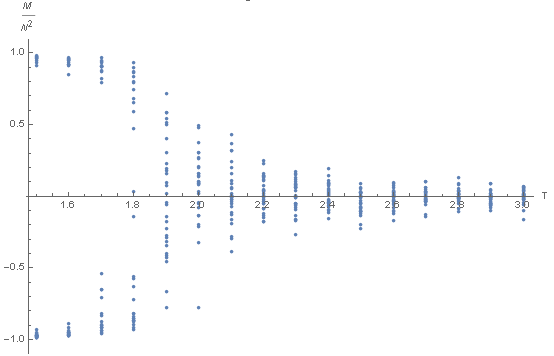
\includegraphics[clip=true,width=\columnwidth]{diagrama_de_fases.png}
    \caption{Magnetización por espín a distintas temperaturas. Las mediciones corresponden al estado estacionario de sistemas de tamaño de red $N=8$. Se obtuvieron errores $\sigma_{desviacion}$ menores a $0.4$. No se colocaron las barras de error para mayor claridad de la imagen.}
     \label{fig:diagrama_de_fases}
\end{figure}

\begin{figure}[h]
    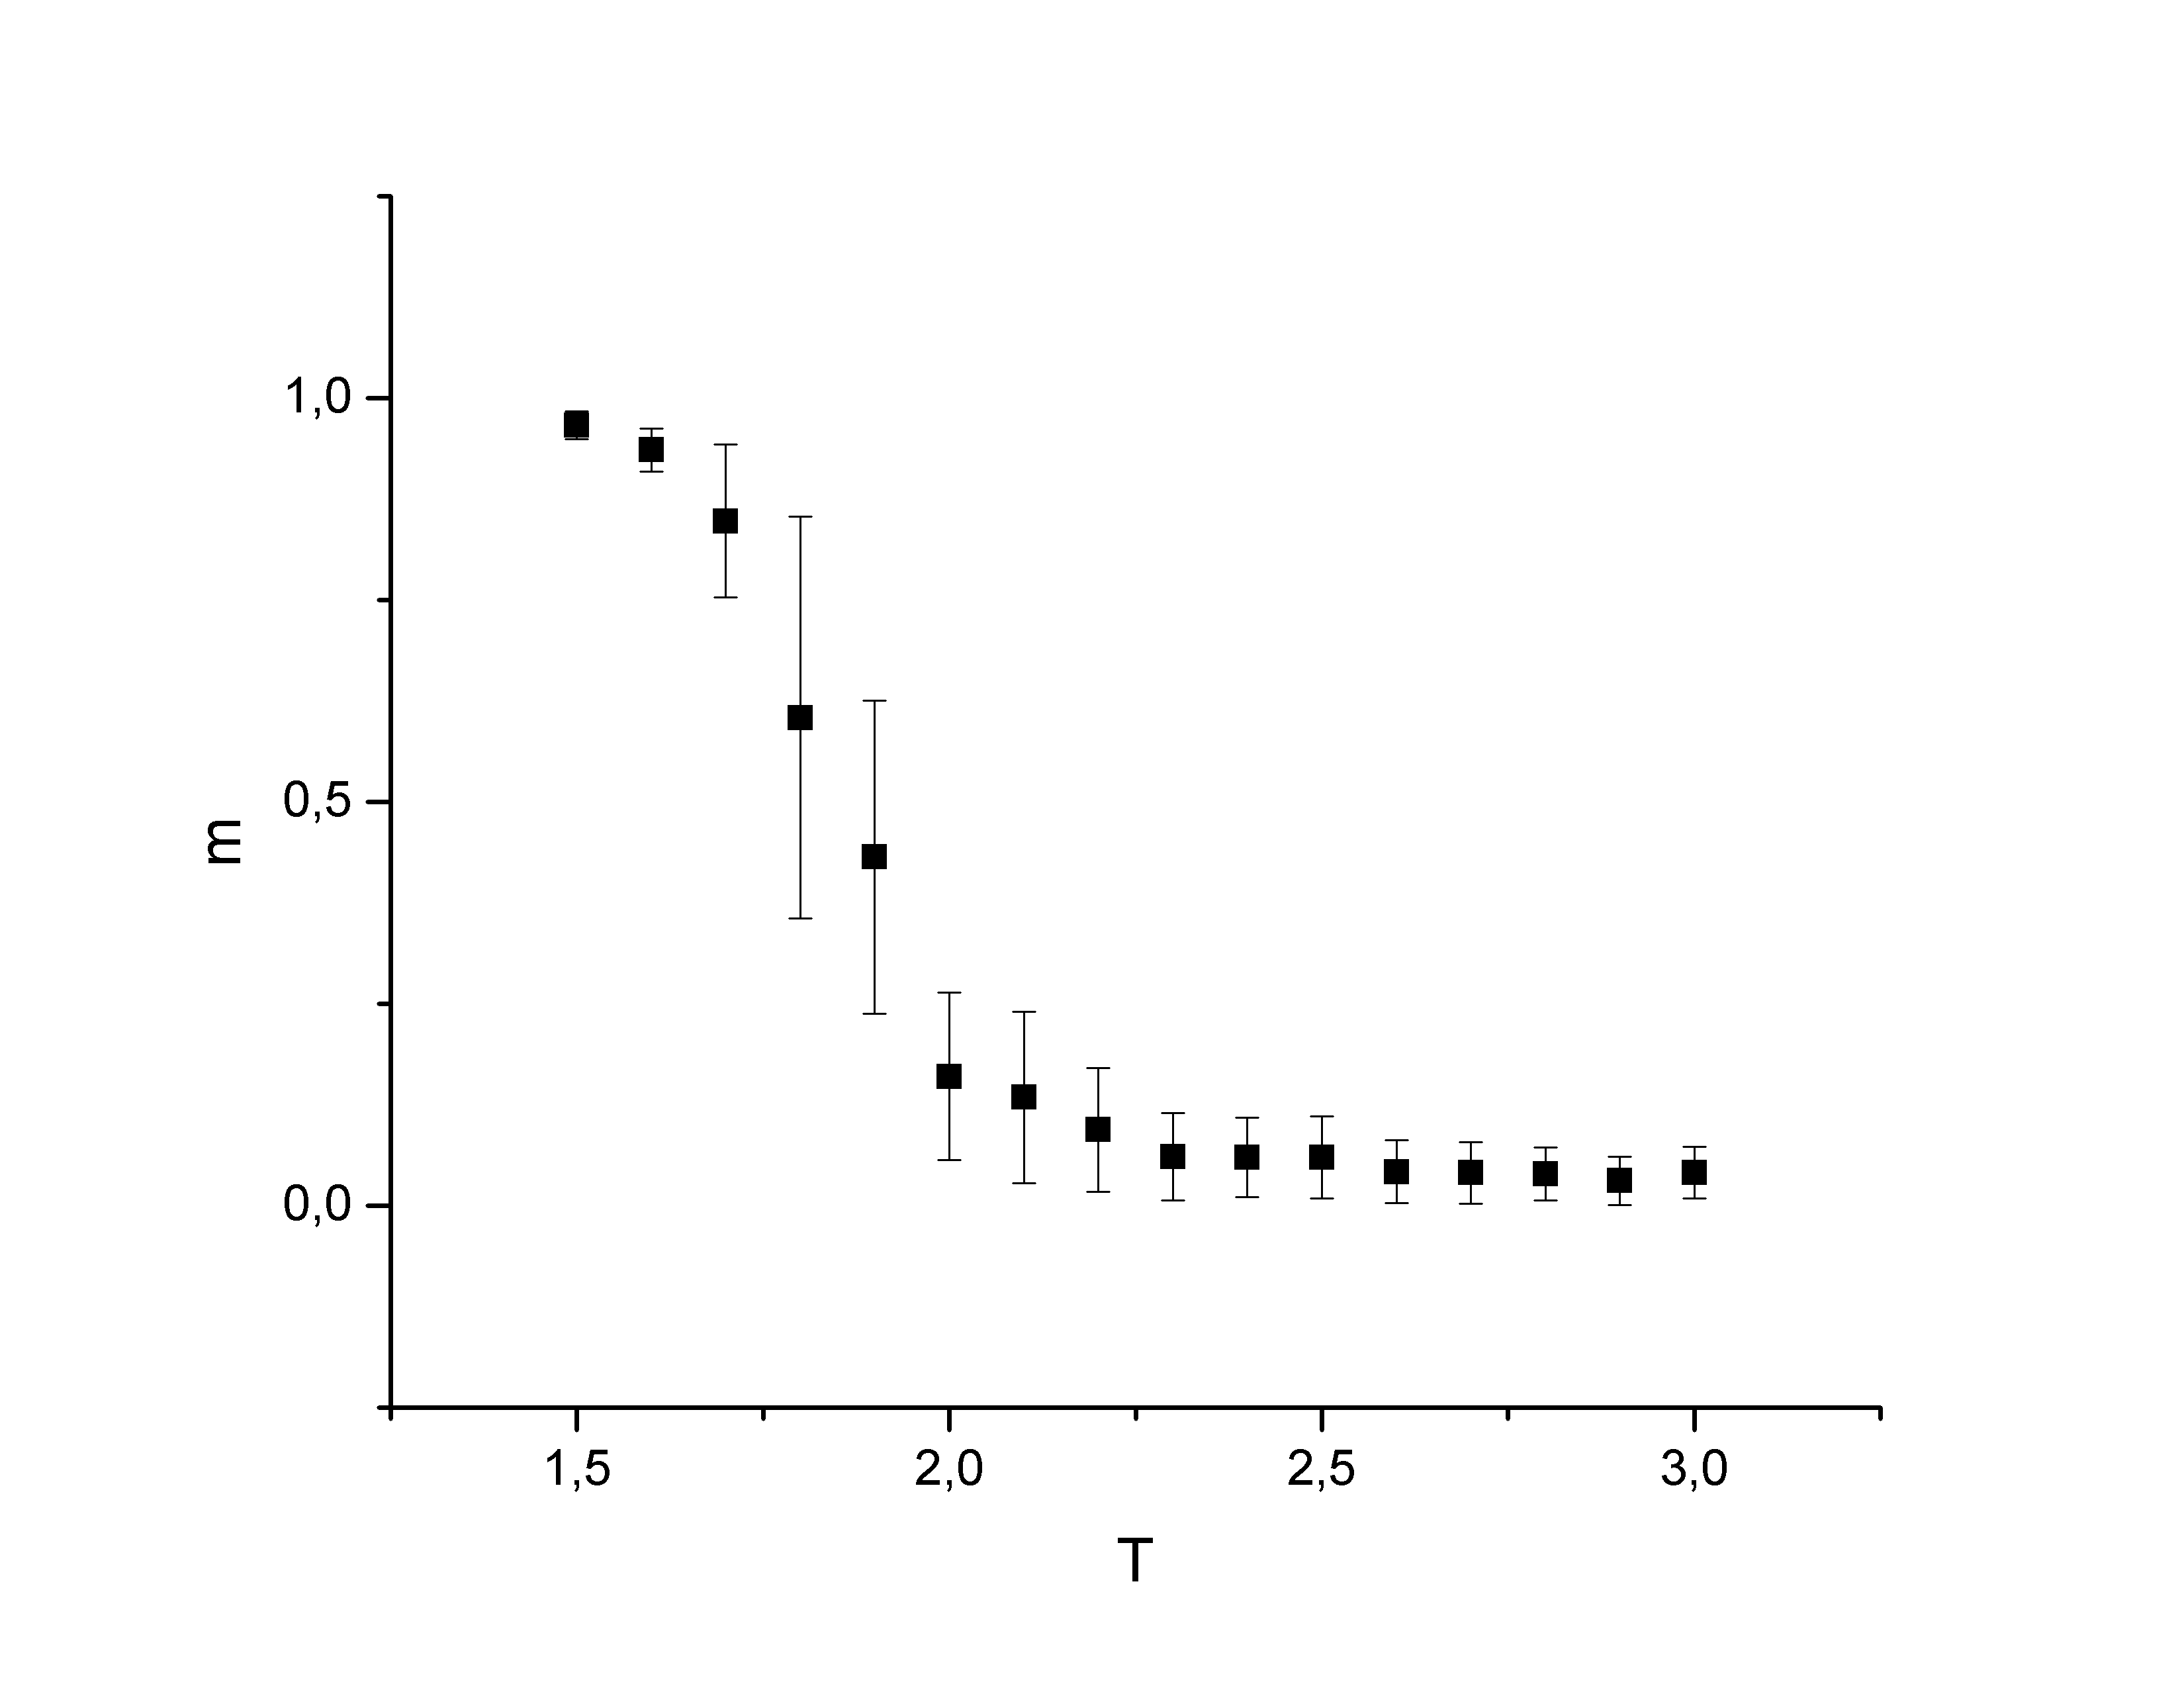
\includegraphics[clip=true,width=\columnwidth]{diagrama_de_fases_pro.png}
    \caption{Diagrama de fases de la magnetización por espín en función de la temperatura.}
     \label{fig:diagrama_de_fases_pro}
\end{figure}


\subsection{Capacidad calorífica}


Se calculó la capacidad calorífica a partir de la expresión \ref{eq:capacidad_calorifica} empleando un ensamble de tamaño $M = 40$ y considerando que el sistema se encuentra en el estado estacionario a partir de $t_{max} = 500$ iteraciones. Se obtuvieron los resultados graficados en la figura \ref{fig:capacidad_calorifica}. Como se mencionó en la introducción, $c$ diverge en $T=T_c$ para una red infinita. Para una red finita, se consideró a $T^*$ tal que $c(T^*)$ es máxima, como una aproximación de la temperatura de Curie. Se obtuvo de este modo $T_c^2 = 2.22$ con una discrepancia del $ 2\%$ respecto al valor teórico. Las diferencias se atribuyen al pequeño tamaño del ensamble y de la red.

\begin{figure}[h]
    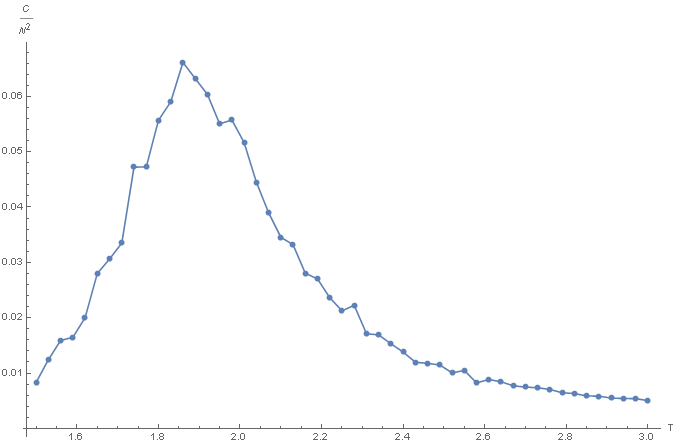
\includegraphics[clip=true,width=\columnwidth]{capacidad_calorifica.png}
    \caption{Capacidad calorífica por espín en función de la temperatura.}
     \label{fig:capacidad_calorifica}
\end{figure}


\bibliography{Radiacion_de_cuerpo_negro}

\end{document}

